\documentclass[tikz,border=10pt]{standalone}
\usetikzlibrary{arrows,intersections}
\definecolor{violet}{RGB}{55,54,112}
\definecolor{redish}{RGB}{189,78,78}
\begin{document}
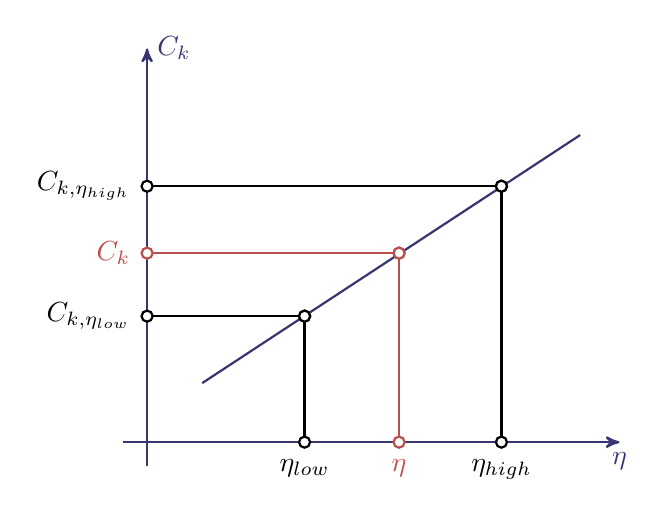
\begin{tikzpicture}[
    thick,
    >=stealth',
    dot/.style = {
      draw,
      fill = white,
      circle,
      inner sep = 0pt,
      minimum size = 4pt
    }
  ]
  \coordinate (O) at (0,0);
  \draw[->, violet] (-0.3,0) -- (6,0) coordinate[label = {below:$\eta$}] (eta);
  \draw[->, violet] (0,-0.3) -- (0,5) coordinate[label = {right:$C_k$}] (C);

     \draw[violet]      (0.7,0.75) -- (5.5,3.9);
     \draw[]  (2,1.6) node[dot] {} -- (2,1.6 |- O) node[dot, label = {below:$\eta_{low}$}] {};
     \draw[]  (4.5,3.25) node[dot] {} -- (4.5,3.25 |- O) node[dot, label = {below:$\eta_{high}$}] {};
     \draw[redish]  (3.2,2.4) node[dot] {} -- (3.2,2.4 |- O) node[dot, label = {below:$\eta$}] {};

     \draw[]  (4.5,3.25) node[dot] {} -- (4.5,3.25 -| O) node[dot, label = {left:$C_{k,\eta_{high}}$}] {};
     \draw[]  (2,1.6) node[dot] {} -- (2,1.6 -| O) node[dot, label = {left:$C_{k,\eta_{low}}$}] {};
     \draw[redish]  (3.2,2.4) node[dot] {} -- (3.2,2.4 -| O) node[dot, label = {left:$C_k$}] {};



\end{tikzpicture}
\end{document}